\documentclass[10pt,a4paper]{report} % Creation d'un rapport avec : 
% taille police : 10 pt
% format : document a4

% Définition des encodages utilisés
\usepackage[T1]{fontenc} % encodage utilisé pour l'impression de caractères (dans le .pdf)
\usepackage[utf8]{inputenc} % encodage utilisé pour la saisie du document (dans le .tex)
\usepackage{lmodern} % utilise la police vectorielle (utile lors d'une impression papier du document) -> c'est plus joli

% Module pour inclure des images 
\usepackage{graphicx} % Pour l'affichage de base

% Module pour inclure des algorithmes en pseudo code
\usepackage[french,onelanguage]{algorithm2e} % Les options permettent d'avoir les mots clés en français

% Module pour insérer des mathématiques
\usepackage{amsmath}
\newcommand\numberthis{\addtocounter{equation}{1}\tag{\theequation}} % Nouvelle commande pour numéroter une équation particulière avec align* (sinon toutes numérotées avec align, ou aucune numérotée avec align*)

% Configuration de la page de garde
\title{Initiation à Latex}
\author{Vous-même}
% Génération d'une image de fond en transparence
\usepackage{eso-pic}
\usepackage{transparent}
\newcommand\BackgroundPic{%
	\put(0,0){%
		\parbox[b][\paperheight]{\paperwidth}{%
			\Logos{images/logo_ensg_transparent}{images/logo_ensg_transparent}
			\vfill
}}
\put(0,0){%
		\parbox[b][\paperheight]{\paperwidth}{%
			\vfill
			\centering
			{
				\transparent{0.1}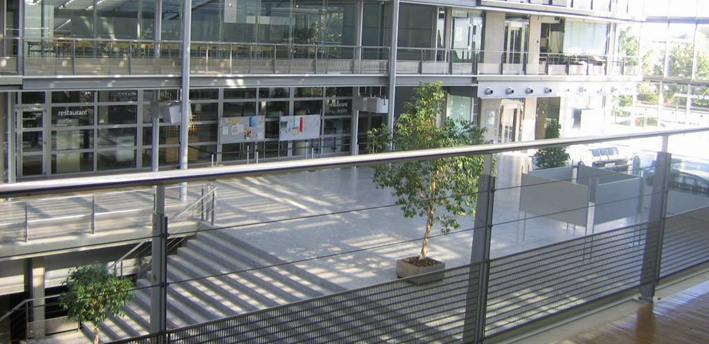
\includegraphics[width=0.9\paperwidth,keepaspectratio]{images/ENSG_hall.jpg}}%
			\vfill
}}
}
% Pour les logos
\newcommand{\Logos}[2]{%
\vspace{1cm}
\begin{center}
\hfill
	\begin{minipage}[c]{0.40\paperwidth}
		\begin{center}
			\includegraphics[width=3.5cm, keepaspectratio]{#1}
		\end{center}
	\end{minipage}
	\hfill
	\hspace*{0.19\paperwidth}
	\begin{minipage}[c]{0.40\paperwidth}
		\begin{center}
			\includegraphics[width=3.5cm, keepaspectratio]{#2}
		\end{center}
	\end{minipage}
	\hfill
\end{center}
}


% Configuration de la langue utilisée (pour les mots clés comme "chapitre", pour le découpage des mots à la fin des lignes...)
\usepackage[french]{babel}

% Module pour inclure des algorithmes implémentés
\usepackage{listingsutf8} % listings peut faire l'affaire. Celui ci gère mieux les problèmes d'encodage. Doit être chargé après babel
\renewcommand{\lstlistingname}{Code} % Permet de modifier le mot utilisé dans la légende

% Module pour régler les marges du document
\usepackage[left=2cm,right=2cm,top=2cm,bottom=2cm]{geometry}


\begin{document}
\AddToShipoutPicture*{\BackgroundPic} % Genere une image de fond
%\AddToShipoutPicture*{\Logos{images/logo_crg}{images/logo_ensg_transparent}}

\maketitle
\ClearShipoutPictureBG % Supprime l'image en fond
\tableofcontents
\listoffigures
\listoftables
\listofalgorithms

\newpage
Mon premier document en Latex. Il a l'air joli, ça me plaît.
Nous allons maintenant structurer le fichier pour faire un joli rapport.

\part{Contexte}
C'est quand même important de commencer par présenter le contexte du travail.
\chapter{Introduction}
Ici nous venons de créer un nouveau chapitre.
\section{Pourquoi cette formation}
Parce que Latex va vous permettre de rédiger un document en équipe, sans se soucier des préférences d'affichage. Latex sera respectueux de l'utilisation de votre système d'exploitation. Il est utilisable que vous soyez sous windows, sous mac ou sous linux.
\subsection{Le lieu}
Durant votre scolarité à l'ENSG, vous allez rédiger bon nombre de rapports. 
\subsubsection{Vertigeo dans tout ça}
Parce que faire de la pub pour la Junior Entreprise, c'est cool.
\paragraph{Rédigé, c'est structuré}
La mise en forme est gérée par Latex, on peut donc en théorie se concentrer sur le contenu du rapport.
\subparagraph{Toujours plus}
Un niveau en dessous du paragraphe. Cela peut être utile dans certaines situations

L'intérêt de cette formation est de vous initier à Latex. Car bien qu'il permet de se concentrer sur le contenu, si son fonctionnement n'est pas compris, ou si personne ne vous a montré un exemple, vous allez passer plus de temps à gérer un problème de mise en forme plutôt qu'écrire du contenu. (Exemple d'une image)

\subsection{Une autre subsection}
Celle ci est vide. Remarquez que le numéro s'est mis à jour.
\section{Quelques conseils}
La table des matières est mise à jour après deux compilations sans modification de la structure entre temps. La première compilation permet à Latex de savoir quelles vont être les entrées. Le deuxième passage va l'afficher.
\subsection*{Structure non numérotée}
Pour ajouter une structure qui n'apparaît pas dans la légende, il suffit de rajouter * après la commande. En faisant ceci, Latex ignorera cette entrée, ce qui signifie pas de numéro, ni de place dans la table des matières. Peut être pratique pour une section Introduction ou Conclusion par exemple.

\subsection{Mettre en valeur des éléments}
Le texte peut être mis en valeur par quelques commandes. Il est possible de \textbf{mettre en gras}, \emph{mettre en italique}.

\section*{Conclusion}
\addcontentsline{toc}{section}{Conclusion}
(Cette entrée apparaît dans la table des matières.)
Au final, nous avons appris quelque chose. Je connais maintenant la base de Latex. Il m'a fallu quelques heures de formation. Je peux désormais rédiger des rapports qui font pro. Je suis content.

\part{Quelques éléments utiles}
\section{Les listes}
Les listes non numérotées : 
\begin{itemize}
	\item Exemple de liste non numérotée
\end{itemize}

Et les listes numérotées : 
\begin{enumerate}
	\item Exemple de liste numérotée
	\item Celle-ci a deux éléments
\end{enumerate}
Notez que le début des paragraphes sont indentés. Ils se retrouvent donc au même \og{}niveau\fg{} que la puce des listes. Ah la langue française\dots
\section{Insérer une image}
Il est possible d'ajouter des images et de les redimensionner par rapport à la dimension du papier, comme la figure \ref{format}.
La référence est mise à jour automatiquement et est associée au label de même nom (se trouvant dans la légende de l'image. Comme pour la table des matières, cela nécessite plusieurs compilations.
\begin{figure}[!ht]
	\begin{center}
		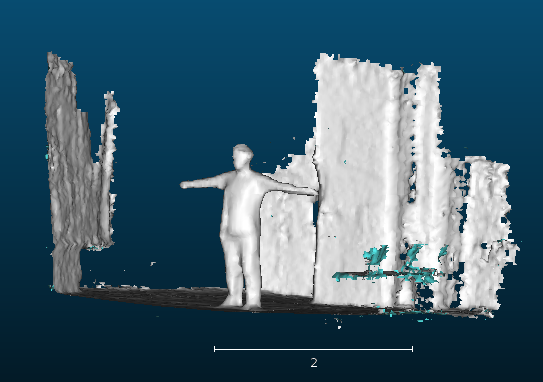
\includegraphics[width=0.50\textwidth, keepaspectratio]{images/format.png}
		\caption{Format obj sans texture \label{format}}
	\end{center}
\end{figure}
  
\section{Insérer un tableau}
\begin{table}[!ht]
	\begin{center}
		\begin{tabular}{rl|c}
			Prenom & Nom      & Promotion \\
			Jean   & Aymare   & 2014      \\
			Jean   & Peuplus  & 2015      \\
			José  & Paledire & 2016      \\
		\end{tabular}
		\caption{Un joli tableau \label{tableau}}
	\end{center}
\end{table}
\section{Insérer des algorithmes}
Voici un exemple d'algorithme en pseudo code : 

\begin{algorithm}[H]
	\SetAlgoLined
	\KwData{Ce document}
	\KwResult{Être capable de rédiger un rapport en Latex }
	initialisation\;
	\While{non à la fin de la formation}{
		Continuer d'écouter\;
		\eIf{compris}{
			Essayer par soit même\;
			Aider ceux qui en ont besoin\;
			}{
			Poser des questions\;
		}
	}
	\caption{Bien suivre la formation}
\end{algorithm}
\section{Insérer du code}
L'option \emph{frame} permet de jouer sur la bordure.
\begin{lstlisting}[language=Python, frame=L, caption={Une imprimante des premiers nombres},label=monImprimante]  % Start your code-block

def printer():
	for i in range(10):
		print(i)
	return true
\end{lstlisting}

\begin{lstlisting}[language=Python, frame=single, caption={Une seconde imprimante des premiers nombres},label=monImprimante2]  % Start your code-block

def printer():
	for i in range(10):
		print(i)
	return true
\end{lstlisting}

\begin{lstlisting}[language=Python, frame=shadowbox, caption={Une troisième imprimante des premiers nombres},label=monImprimante3]  % Start your code-block

def printer():
	for i in range(10):
		print(i)
	return true
\end{lstlisting}


\section{Insérer des formules mathematiques}
Il est possible d'écrire des formules mathématiques intégrées dans le texte, comme \begin{math}(a-b)^2=a^2-2ab+b^2\end{math} ou en utilisant la notation condensée $(a+b)^2=a^2+2ab+b^2$.

De la même façon, il est possible de séparer les formules mathématiques pour les rendre plus visibles :
\begin{displaymath}
	det \begin{pmatrix}
	\alpha & \beta \\
	\gamma & \delta
	\end{pmatrix} = \alpha\delta - \gamma\beta 
\end{displaymath} ou dans sa notation abrégée : 
$$
\begin{vmatrix} 
	a & b \\
	c & d 
\end{vmatrix} = ad - cb
$$

On peut même utiliser une structure similaire à la précédente et qui permet de numéroter les équations : \begin{equation}
\sin x=\sum_{k=0}^{\infty}\frac{(-1)^k}{(2k+1)!}x^{2k+1}
\end{equation}
\begin{align*}
	\int_a^b x^2 \, \mathrm dx & = {\lbrack \frac{x^3}{3} \rbrack}_a^b                     \\
	                           & = \frac{b^3}{3} - \frac{a^3}{3}                           \\
	                           & = \frac{b^3-a^3}{3} \numberthis \label{resultatIntegrale} 
\end{align*}
L'équation \eqref{resultatIntegrale} montre que le résultat de l'intégrale est calculable.
\medbreak
Latex génère aussi les flèches pour les vecteurs. Avec ça, on a quasiment tout ce qu'il nous faut pour faire des maths.
$$
\overrightarrow{\nabla }=\frac{\partial }{\partial x}\overrightarrow{i}+\frac{\partial }{\partial y}\overrightarrow{j}+\frac{\partial }{\partial z}
\overrightarrow{k}
$$


\end{document}


